\documentclass[tikz,convert={density=150,size=600,outext=.png}]{standalone}
\usetikzlibrary{shapes, calc, arrows, fit, positioning, decorations, patterns, decorations.pathreplacing, chains, snakes}

\begin{document}
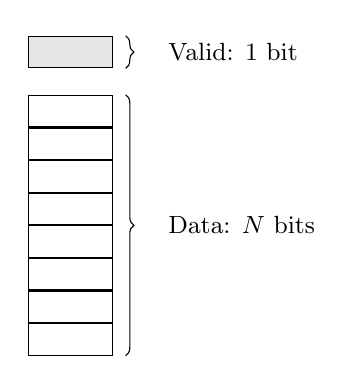
\begin{tikzpicture}[inner xsep=1pt, inner ysep=0.2cm, node distance=0cm, font=\small, scale=0.8]
    \node[draw, text width = 1cm, fill=black!10] (valid-bit) {};
    \node[draw, text width = 1cm, below of=valid-bit, node distance = 0.75cm] (data1) {};
    \node[draw, text width = 1cm, below =of data1.south] (data2) {};
    \node[draw, text width = 1cm, below =of data2.south] (data3) {};
    \node[draw, text width = 1cm, below =of data3.south] (data4) {};
    \node[draw, text width = 1cm, below =of data4.south] (data5) {};
    \node[draw, text width = 1cm, below =of data5.south] (data6) {};
    \node[draw, text width = 1cm, below =of data6.south] (data7) {};
    \node[draw, text width = 1cm, below =of data7.south] (data8) {};
    \draw[decorate, decoration={brace, amplitude=3pt}] ([xshift=0.2cm] data1.north east) -- ([xshift=0.2cm] data8.south east) node[midway, auto, xshift=0.5cm] {Data: $N$ bits};
    \draw[decorate, decoration={brace, amplitude=3pt}] ([xshift=0.2cm] valid-bit.north east) -- ([xshift=0.2cm] valid-bit.south east) node[midway, auto, xshift=0.5cm] {Valid: 1 bit};
\end{tikzpicture}
\end{document}
